\documentclass[../main.tex]{subfiles}

\graphicspath{{pictures/}{../pictures/}}

\chapterimage{chapter_head_2.pdf} % Chapter heading image

\begin{document}
	\chapter{Basic Syntax}
	
	%----------------------------------------------------------------------------------------
	%	Basic Syntax
	%----------------------------------------------------------------------------------------
	
	\section{Types}
	
	Much of programming is about the receiving, manipulating, and sending of data.  Since C is a typed language, it needs to know how to interpret the data that you are working with.  In many cases, the underlying bits that are actually being stored are the same.  However, based on the type assigned to that data, the C compiler will interpret it differently.  C can't really tell the difference between 41 and the letter 'A' (which has the ASCII value of 41).  Its up to you as the programmer to specify if the data is an integer or if its a character.
	
	There are a few basic data types you'll encounter in C.	
	\begin{itemize}
		\item \textbf{int}		-	Represents whole numbers.
		\item \textbf{char}		-	Represents a single character.
		\item \textbf{float}	-	Represents numbers with decimal points (single precision).
		\item \textbf{double} 	-	Represents numbers with decimal points (double precision).
	\end{itemize}

	The platform that a program is compiled for can affect the number of bytes that a data type requires.  While most of today's platforms are 64-bit, there are still a few 32-bit systems out there.  If the max or min size of a data type is a concern to you, you'll want to be sure you know the size of that type on the platform your code will be compiled for.
	%----------------------------------------------------------------------------------------
	%	Integer
	%----------------------------------------------------------------------------------------	
	\subsection{Integers}
	
	By default, an \textit{int}\index{int} utilizes 4 bytes on both the 32-bit and 64-bit platforms. However, there are a couple of qualifiers that can affect how the data is interpreted as well as how many bytes are used.  
	\begin{itemize}
		\item \textbf{short}	-	Utilizes 2 bytes (16 bits).
		\item \textbf{long}		-	Utilizes 4 bytes on a 32 bit platform and 8 bytes on a 64 bit platform.
		\item \textbf{long long}-	Utilizes 8 bytes on a 32 bit platform and 8 bytes on a 64 bit platform.
		\item \textbf{signed}	-	Integers are \text{signed} by default meaning they utilize two's complement to represent positive and negative numbers.  You do not need to specify \textit{signed} but can for greater clarity for someone reading your code.
		\item \textbf{unsigned}	-	As an \textit{unsigned} integer, there is no sign bit.  Therefore you can store larger positive numbers but you cannot store negative numbers.\\
	\end{itemize}
	
	\lstinputlisting[caption={\lstname}]{src/02-integer-32bit.c}
	
	\begin{lstlisting}[language=bash, numbers=none]
		$ file 02-integer-32bit
		02-integer-32bit: ELF 32-bit LSB shared object, Intel 80386
		
		$ ./02-integer-32bit 
		Number of Bytes:
		short int: 2
		int: 4
		long int: 4
		long long int: 8
		
		Value of signed   short: -275
		Value of unsigned short: 65261
		
		Min signed int: -2147483648
		Max signed int: 2147483647
		
		Min unsigned int: 0
		Max unsigned int: 4294967295
	\end{lstlisting}
	
	As you can see with the \textit{file} command, 02-integer-32bit has been compiled as a 32-bit binary.  Notice that an \textit{int} and \textit{long int} are both 4 bytes but a \textit{long long int} is 8 bytes.  
	
	Also notice on line 11 that I assign the value of -275 to \textit{si} which is a \textit{signed short int} and it prints out just fine on line 14.  However, when I print it out a second time on line 15 I cast it as an \textit{unsigned short int}.  Under the hood, the bits haven't changed; how they were interpreted did.  -275 is actually 1111111011101101 in binary.  The left-most bit (most significant bit) is the \textit{sign} bit.  When cast as an \textit{unsigned short int}, this bit is not longer interpreted as a signed bit which is why we now get a positive number.  I point this out only because it is important to note that you as the programmer need to understand the data you are working with because C only pays attention to whether or not you declared it as \textit{signed}\index{signed} or \textit{unsigned}\index{unsigned}.  To further demonstrate this, I've printed out the max and min value that a signed integer and an unsigned integer can hold.\\
	
	\lstinputlisting[caption={\lstname}]{src/02-integer-64bit.c}
	
	\begin{lstlisting}[language=bash, numbers=none]
	$ file 02-integer-64bit
	02-integer-64bit: ELF 64-bit LSB shared object, x86-64
	
	$ ./02-integer-64bit 
	Number of Bytes:
	short int: 2
	int: 4
	long int: 8
	long long int: 8
	\end{lstlisting}
	
	Notice this 02-integer-64bit is compiled as a 64-bit executable.  In this case, an \textit{int} is still 4 bytes but a \textit{long int} is now 8 bytes allowing you to store much larger numbers.  If you have a requirement to store very large numbers and you're program needs to run on both 32 bit and 64 bit, a \textit{long long int} provides consistency by using 8 bytes for both.
	
	%----------------------------------------------------------------------------------------
	%	Characters
	%----------------------------------------------------------------------------------------

	\section{Characters}
	
	A \textit{char}\index{char} within C typically requires just a single byte to store a single character.  This is based upon the fact that the \textit{char} was meant to store the ASCII\index{ASCII} value which only required 7 bits.  Depending upon the type of project you are working on, this may or may not be sufficient. Below is the ASCII chart \ref{fig:ascii} as printed out by running the \textit{ascii} command on the terminal.  Notice the values only go upto 127.
	
	\begin{figure}[h]
		\centering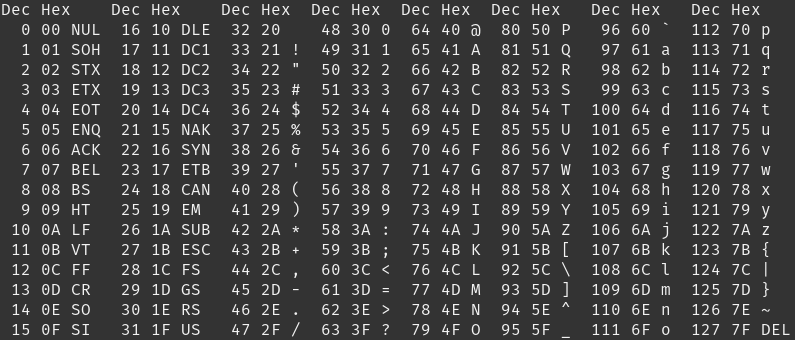
\includegraphics[scale=0.5]{ascii.png}
		\caption{ASCII Chart}
		\label{fig:ascii} % Unique label used for referencing the figure in-text
	\end{figure}
	
	Obviously the ASCII chart was built for the English language.  When not sufficient, there are ways of using an \textit{unsigned int} and \textit{UTF-8} encoding instead.  I will not be going into this but if it interests you, I suggest checking out articles such as \href{https://www.cprogramming.com/tutorial/unicode.html}{https://www.cprogramming.com/tutorial/unicode.html}.\\
	
	\lstinputlisting[caption={\lstname}]{src/02-character1.c}
	
	\textbf{Line 2}: Here I import \textit{ctype.h}.  Doing so gives me access to a number of functions and macros pertaining to the use of characters.\\
	\textbf{Line 7}: Here I declare a \textit{char} and give it the value of \textit{a}.  Notice it holds a single character and I use single quotes.\\
	\textbf{Line 8}: Here I use the function toupper which has a function \textit{declaration} of \textbf{int toupper(int c);}.  This is our first indication that under the hood, a \textit{char} is treated very much like an \textit{int}.\\
	\textbf{Line 14}: Here I use the function \textit{isalpha} to test to see if the character is alphabetic.\\
	\textbf{Line 22}: Here I use the function \textit{isdigit} to test to see if the character is a digit.\\
	
	By typing '\texttt{man 3 toupper}' on the terminal, I am presented with the manual page describing the C \textit{toupper} function:\\
	
	\begin{figure}[h]
		\centering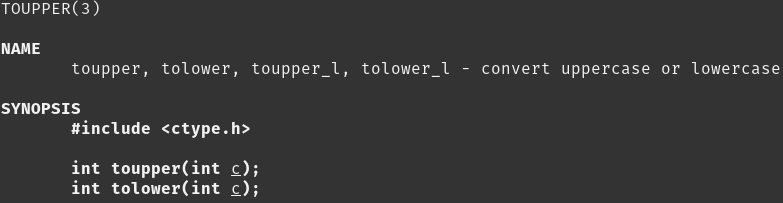
\includegraphics[scale=0.5]{toupper.png}
		\caption{toupper}
		\label{fig:toupper} % Unique label used for referencing the figure in-text
	\end{figure}

	Likewise, I can view the manpage for \textit{isdigit} by typing '\texttt{man 3 isdigit}'.\\
	
	\begin{figure}[h]
		\centering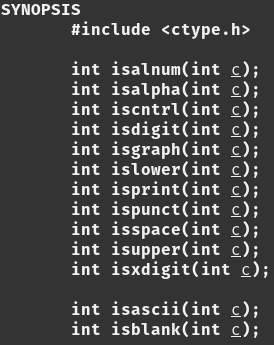
\includegraphics[scale=0.5]{isalpha.png}
		\caption{isalpha, isdigit}
		\label{fig:isapha} % Unique label used for referencing the figure in-text
	\end{figure}

	%----------------------------------------------------------------------------------------
	%	Floats
	%----------------------------------------------------------------------------------------
	
	

\end{document}